%!TeX encoding = utf8
%!TeX spellcheck = it_IT
%!TeX source = ../relazione.tex

\begin{centering}
	\emph{Dire brevemente che facciamo una simulazione di una particella sul cerchio}
\end{centering}

Innanzitutto vediamo che per $\beta=5$, $\chi=1$ e $N_t=200$ estraiamo dei campi fatti come quello in figure \ref{fig:field}
\begin{figure}[htbp]
	\centering
	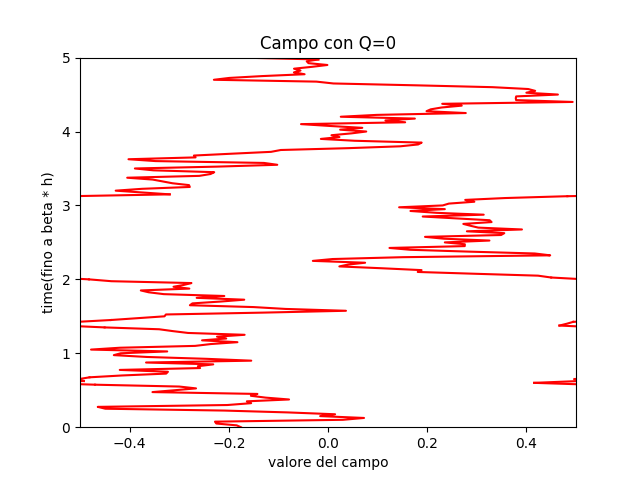
\includegraphics[width=1\linewidth]{3/Q=0_field}
	\caption{Esempio di una configurazione di campo (con $N_t=200$)}
	\label{fig:field}
\end{figure}

una markov chain del mio problema è rappresentata in figure \ref{fig:windingnumber}
\begin{figure}[htbp]
	\centering
	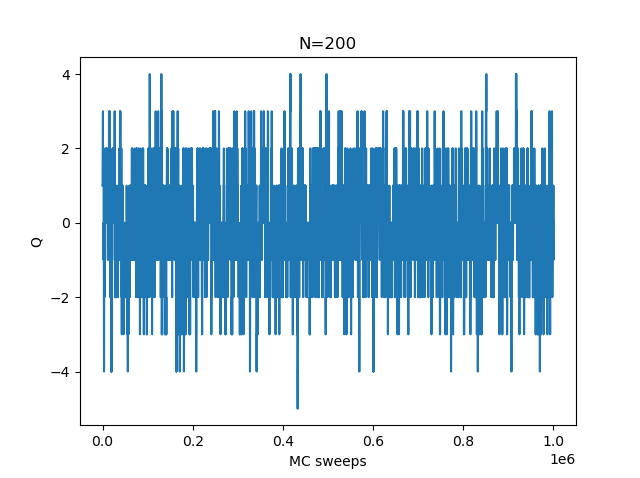
\includegraphics[width=1\linewidth]{3/N=200_winding_number}
	\caption{Ho estratto un milioni di campi e calcolato il winding number (quante volte si avvolgono intorno alla circonferenza)}
	\label{fig:windingnumber}
\end{figure}

E facciamo vedere che sappiamo calcolare il tempo di autocorrelazione ($\tau=$ runnare il codice) come si vede in figura \ref{fig:autocorrelation}, sono stato attendo e ho integrato fino al plateau.

\begin{figure}[htbp]
	\centering
	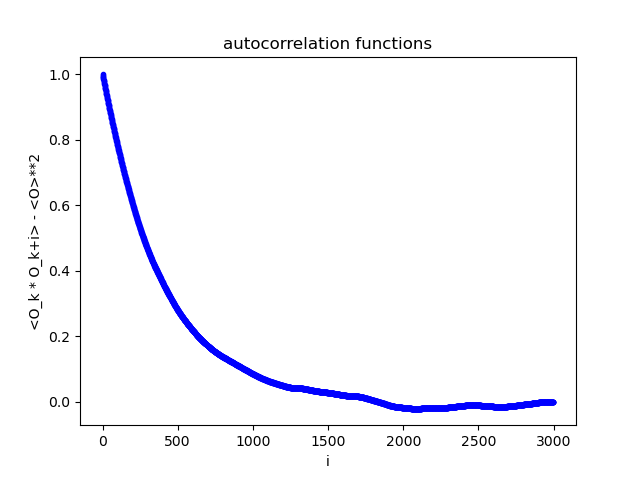
\includegraphics[width=1\linewidth]{3/autocorrelation_functions}
	\caption{funzioni di autocorrelazione per il winding number}
	\label{fig:autocorrelation}
\end{figure}

A questo punto abbiamo impostato bene il nostro problema e vediamo che cambiando N incontro un critical slowing down, che si vede bene calcolando il tempo di autocorrelazione in figura \ref{fig:tau_criticalslowingdown}

\begin{figure}[htbp]
	\centering
	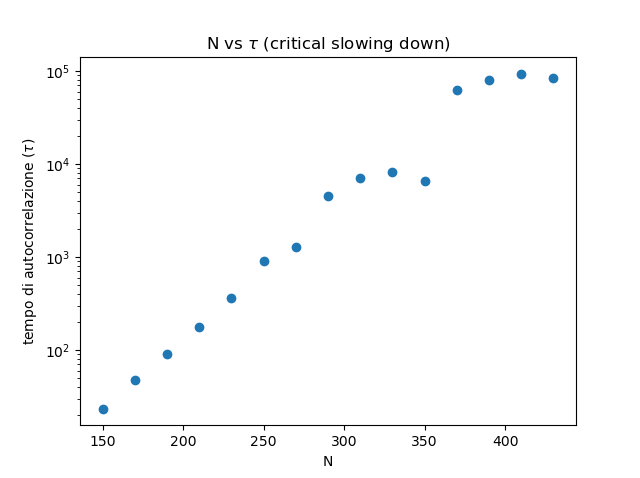
\includegraphics[width=1\linewidth]{3/tempo_di_autocorrelazione_-_critical_slowing_down}
	\caption{A temperatura fissata, a meno di fluttuazioni è più difficile cambiare Q per N crescente, quindi la suscett: $<Q^2>$ diminuisce e il tempo di autocorrelazione aumenta; $10^6$ misure}
	\label{fig:tau_criticalslowingdown}
\end{figure}

infine posso risolvere il problema con il taylor update ogni sweep del reticolo (figura \ref{fig:tau_taylor}).

\begin{figure}
	\centering
	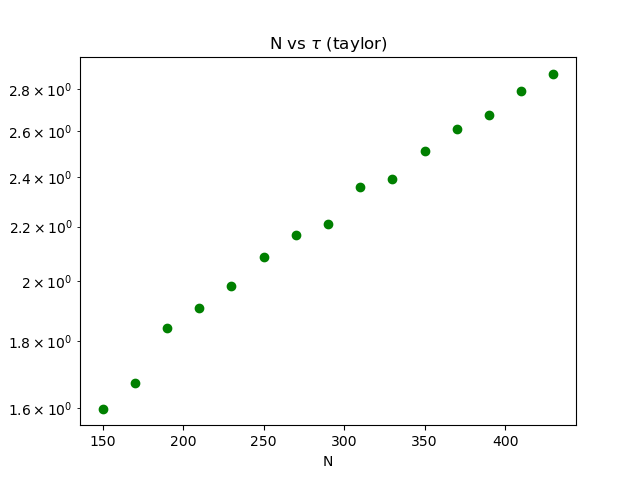
\includegraphics[width=1\linewidth]{3/tempo_di_autocorrelazione_-_taylor}
	\caption{Tempo di autocorrelazione implementando il taylor method; $10^5$ o forse $10^6$ misure}
	\label{fig:tau_taylor}
\end{figure}
